Kitāb Mu'jam al-Buldān \cite{Yaqut} "Dictionary of Countries" was written by Yāqūt Shihāb al-Dīn ibn-ʿAbdullāh al-Rūmī al-Ḥamawī
between 1224 and 1228.

The Gazetteer is a "comprehensive index of places and places descriptions, mainly in the Muslim World ...
he (Yāqūt) depicted a semi-anachronistic look at the Muslim Caliphate in the 7th-10th centuries
"~\cite{YaqutRB}
At the time of writing, there's no exact number for the places detailed in the book, but there are at least 12,400 entries.

Some projects however distinguish multiple places, if they're mentioned within a different entry, lacking
their own dedicated one.~\cite{AlTurayya}.

Example entries are shown on figure~\ref{fig:yaqut-entries}


\begin{figure}[h] % [h] attempts to place figure here, other options like [t]op, [b]ottom
    \centering % Centers the figure horizontally
    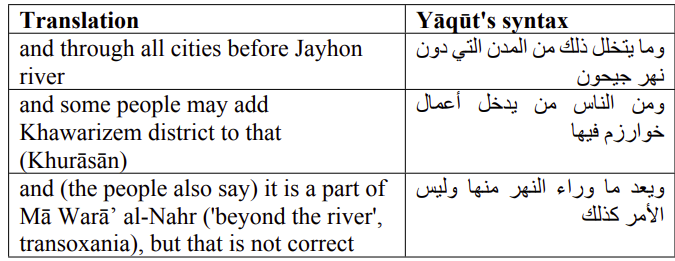
\includegraphics[width=0.7\linewidth]{figures/yaqut-with-translation} % Include the image with desired width
    \caption{Original, Arabic entries from Kitāb Mu'jam al-Buldān with their corresponding English tranlations~\cite{YaqutRB}} % Add a caption
    \label{fig:yaqut-entries} % Assign a label for referencing the figure in text
\end{figure}.

\subsection{Parsed Dataset - Places}
The layout of the gazetteer is highly structured, therefore, researchers were able to create a rule based method to parse
and expose the data in a tabular database~\cite{YaqutRB}.
This database provides serves as the primary datasource for this thesis.

\begin{figure}[h] % [h] attempts to place figure here, other options like [t]op, [b]ottom
    \centering % Centers the figure horizontally
    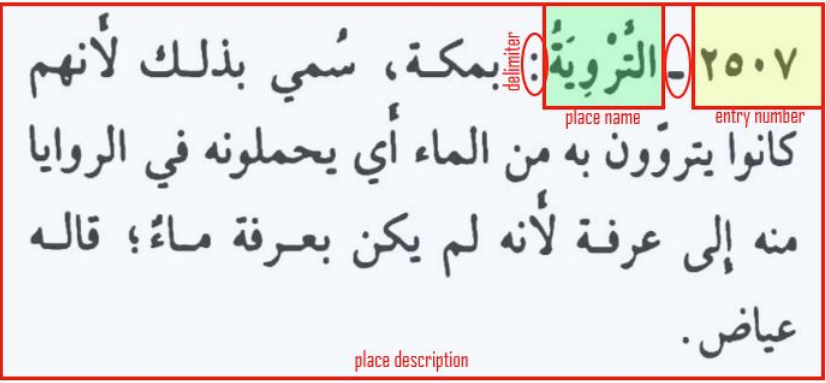
\includegraphics[width=0.8\linewidth]{figures/yaqut-layout} % Include the image with desired width
    \caption{Example of Muʿjam al-Buldān entry ~\cite{YaqutRB}} % Add a caption
    \label{fig:yaqut-structure} % Assign a label for referencing the figure in text
\end{figure}.

The primary, parsed datasource provided the following information:
\begin{itemize}
    \item Latitude
    \item Longitude
    \item Wikidata ID
    \item al-Turayyā ID~\cite{AlTurayya}
    \item Name (Arabic)
    \item Name (English)
    \item Type (lower hierarchy)
    \item Type (upper hierarchy)
    \item Metropolitan ID (reference to another place in the dataset)
    \item District ID (reference to another place in the dataset)
    \item Provincial ID (reference to another place in the dataset)
\end{itemize}


The only fields guaranteed to have data were the Arabic name and the unique identifier assigned based on the corresponding al-Turayyā gazetteer~\cite{AlTurayya}.

\subsubsection{al-Turayyā ID}
The IDs correspond to the database entries partially backing the al-Turayyā gazetteer project.
Namely, al-Turayyā used the same IDs to identify the OCR scanned entries.
A small caveat is that~\cite{YaqutRB} occasionally parsed multiple place descriptions from the same entry,
therefore, these entries have additional suffixes after the al-Turayyā ID to keep them unique.

\subsubsection{Wikidata ID}
Some more well known and easily identifiable place entries such as Baghdad were already enriched with Wikidata~\cite{Wikidata} IDs.
This information was initially used to build some graphs, but later iterations forewent its use due to the unreliability.
As an example, the entry for Mecca, which is a highly central and important node had the Wikidata ID of Q3289054
which refers to a city in the United States, not to the Saudi Arabian city.

\subsubsection{Categories}
The rule based parsing system also attempts to assign a category to each place entry.
The categories are selected from a pre-defined hand verified list.

The categories are split into a two level hierarchy.
For example, the level one category "town" has multiple sub-categories, like
village, small town, neighboring villages or abodes.

However, not all entries necessarily will have a secondary category.
In total there are 96 distinct categories.

\subsection{Parsed Dataset - Distances}
The other important block of data available in the parsed dataset are the distances.
There are over a thousand entries parsed from the original book, that express some spatial relationship
between two places.

The dataset this thesis works with, already contains this information in kilometres, but it is important
to keep in mind that the kilometer values provided are highly varying in terms of accuracy. This
is due to the fact that the original entries defined distance in terms of various non-standard methods
such as days of walking, travelling on camel back and so on.


